\chapter{Theory} \label{cha:theory} %\thispagestyle{main}
This chapter explains the overall theory that forms the fundamental principles of this project. Initially, the characteristics of ultrasound will be explained from an acoustics standpoint. Then, a brief overview of systemic circulation is explained in vivo. Lastly, the various types of flow meters are outlined with their strengths and weaknesses.
\section{Ultrasound}
\begin{figure}[htbp]
	\centering
	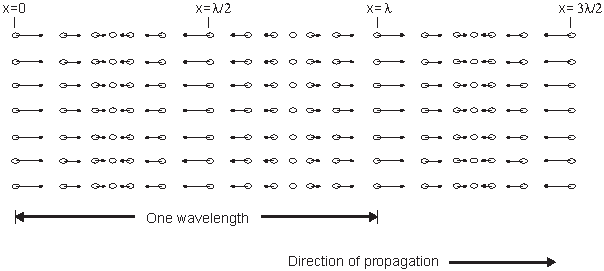
\includegraphics[width=\textwidth]{2_plane_wave_jensen-cropped.pdf}
	\caption[Particle displacement for a propagating ultrasound wave]{Particle displacement for a propagating ultrasound wave \cite{JensenUltrasoundBook}}
	\label{fig:2_planewave_jensen}
\end{figure}
\gls{us} is a technology that transmits sound wave with frequencies above the audible range (\qtyrange[range-units = single]{20}{20e3}{\hertz}) to mechanically vibrate matter. The particles in the medium would be at rest and distributed uniformly before any disturbance. The wave propagates as a disturbance and the particles oscillate around their mean position due to the presence of the ultrasonic wave. Typically, the \gls{us} frequency-band used in clinical settings are from \qtyrange[range-units = single]{1}{15}{\mega\hertz} \cite{Szabo_UltrasoundBook_2}. Certain specialist applications, such as eye, skin, and small animal imaging may use ultrasound frequencies at or above \qty{20}{\mega\hertz.} \cite{Winckler2012}. The trade-off with very high-frequency ultrasound balances increased resolution with reduction in penetration depth. For blood velocity estimation or echocardiography, moderate penetration is more important than resolution. Thus, the frequency used is most often at \qty{10}{\mega\hertz} or less. \Cref{fig:2_planewave_jensen} visualizes the propagation of a plane wave in matter. The oscillation occurs parallel to the wave's direction, making it longitudinal, and the disturbance will propagate with the variable $c$, which is determined by the medium and is given by \cref{eq:2_velocity_c}.
\begin{equation} \label{eq:2_velocity_c}
	c = \sqrt{\frac{1}{\rho_{0} \kappa_{S}}}
\end{equation}
Where $\rho_{0}$ is the mean density (\unit{\kilogram\per\meter\cubed}) and $\kappa_{S}$ is the \gls{adiabatic} compressibility (\unit{\meter\squared\per\newton}). Since in the majority of cases, the propagation of ultrasound is linear, it is assumed in this work. The acoustic pressure of the harmonic plane wave is expressed by \cref{eq:2_acoustic_pressure}. \raggedbottom
\begin{equation} \label{eq:2_acoustic_pressure}
	p(t,z)=p_{0} e^{j(\omega t - k z)}
\end{equation}
And propagates along the $z$-axis. $\omega$ is the angular frequency, $k$ is the wave number and is expressed by $k=\sfrac{\omega}{c}=\sfrac{2\pi}{\lambda}$, and $_{0}$ is the acoustic pressure amplitude. A spherical wave is expressed by \cref{eq:2_spherical_wave}
\begin{equation} \label{eq:2_spherical_wave}
	p(t,r)=p_{0} e^{j(\omega t - k r)}
\end{equation}
Where $r$ is radial distance and is defined in a polar coordinate system. For each time instance, the acoustic pressure $p(t,r)$ is constant over a fixed radial position. In this scenario, the pressure amplitude is given by $p_{0}(r) = \sfrac{k_{p}}{r}$, where $k_{p}$ is a constant since the energy of the outgoing wave must be constant.  Particle speed $u$ is dependent on the pressure caused by a wave expressed by \cref{eq:2_particle_speed}
\begin{equation} \label{eq:2_particle_speed}
	u = \frac{p}{Z}
\end{equation}
Where $Z$ is the characteristic acoustic impedance, defined as the ratio of acoustic pressure to particle speed at a given position in the medium and is expressed by \cref{eq:2_acoustic_impedance}.
\begin{equation} \label{eq:2_acoustic_impedance}
	Z = \rho_{0} c
\end{equation}

Characteristic acoustic impedance $Z$ is one of the most significant variables in the characterization of propagating plane waves. Reference values for density, speed of sound, and characteristic acoustic impedance can be seen in \cref{tab:2_density_tissue}.

\begin{table}[htbp]
	\centering
	\caption[Approximate density, sound speed, and acoustic impedance of human tissue types]{Approximate density, sound speed, and acoustic impedance of human tissue types \cite{JensenUltrasoundBook}}
	\label{tab:2_density_tissue}
	\sisetup{range-phrase=--,range-exponents = combine}
	\begin{tblr}[]{
		colspec = {XSSS},
		row{1} = {guard,m,font=\small\bfseries},
		}
		\toprule
		Medium & {Density ($\rho_{0}$)\\\unit[per-mode = symbol]{\kilogram\per\meter\cubed}} & {Speed of sound ($c$)\\\unit[per-mode = symbol]{\meter\per\second}} & {\textbf{Acoustic impedance ($Z$)}\\\unit[per-mode = symbol]{\kilogram\per\meter\squared\per\second}} \\ \midrule
		Air             & 1.2     & 333            & 0.4e3       \\
		Blood           & 1.06e3    &    1566        &  1.66e6     \\
		Bone            & \numrange{1.38e3}{1.81e3}  &   \numrange{2070}{5350}       & \numrange{3.75e6}{7.38e6} \\
		Brain           &  1.03e3       & \numrange{1505}{1612}  & \numrange{1.55e6}{1.66e6} \\
		Fat             &  0.92e3  &  1446 & 1.33e6 \\
		Kidney          &  1.04e3  & 1567 & 1.62e6 \\
		Lung            &  0.4e3  &  650  & 0.26e6 \\
		Liver           &  1.06e3  &  1566  & 1.66e6 \\
		Muscle          &  1.07e3  & \numrange{1542}{1626} & \numrange{1.65e6}{1.74e6} \\
		Spleen          &  1.06e3  & 1566 & 1.66e6 \\
		DI				&  1e3  & 1480 & 1.48e6 \\ \bottomrule
	\end{tblr}
\end{table}

In the following sections, various acoustic wave phenomena will be briefly described.

\subsection{Scattering}
A wave propagating through a medium continues in the same direction until it encounters a new medium. When this occurs, a portion of the wave is transmitted into the new medium with a change in direction. Because the scattered wave is the result of several contributors, it is necessary to define it statistically. The amplitude distribution is Gaussian \cite{JensenUltrasoundBook} and can thus be fully described by its mean and variance. The mean value is zero because the dispersed signal is caused by variances in the acoustic characteristics in the tissue. The correlation between multiple data is what allows ultrasound to determine blood velocities. Because minor movements have a significant correlation, it is feasible to discover alterations in location by comparing sequential measurements of moving structures, such as blood cells. In medical ultrasound, only one transducer is used to transmit and receive, and only the backscattered signal is analysed. The power of the scattered signal is defined by the scattering cross-section, which in small cases means a uniform intensity $I_{i}$, and is expressed by \cref{eq:2_scatter_power}.
\begin{equation} \label{eq:2_scatter_power}
	P_{s} = I_{i} \sigma_{s c}
\end{equation}
Where $\sigma_{s c}$ is the scattering cross-section in square meters. The backscattering cross section is material dependant and determines the intensity of the scattering. If the dispersed energy is evenly emitted in all directions, the scattered intensity is given by \cref {eq:2_scatter_intensity}.
\begin{equation} \label{eq:2_scatter_intensity}
	I_{s} = \frac{P_{s}}{4 \pi R^{2}} = \frac{\sigma_{sc}}{4 \pi R^{2}} \cdot I_{i}
\end{equation}
Where $R$ is the distance to the scattering region \cite{JensenUltrasoundBook}. This results in a spherical wave. A transducer with radius $r$ gives the power $P_{r}$, presuming the attenuation and focus are neglected, and is expressed by \cref{eq:2_transducer_r_power}.
\begin{equation} \label{eq:2_transducer_r_power}
	P_{r} = I_{s} \pi r^{2} = \sigma_{s c} \frac{r^{2}}{4 R^{2}} \cdot I_{i}
\end{equation}

The backscattering coefficient, which characterizes scattering from a volume of scatterers, is another measure of scattering strength. It is defined as the average received power per steradian volume of scatterers when flooded with plane waves of unit amplitude and the unit is \unit{1\per\centi\meter\steradian}. Back-scattering coefficients in the blood are significantly lower than the backscattering coefficients from various tissue types. This poses a challenge when estimating blood flow close to tissue vessel walls \cite{ShungScattering1992,JensenUltrasoundBook}.

\subsection{Attenuation}
The ultrasonic wave will be reduced as it propagates through the tissue due to absorption and scattering. The attenuation in tissue is frequency dependent, with greater attenuation with increasing frequency. Because of absorption and dispersion, the ultrasonic wave will be attenuated as it travels through the tissue. The relationship between attenuation, distance travelled, and frequency is often linear. Attenuation in the tissue occurs as a result of both dispersion, which spreads energy in all directions, and absorption, which turns it into thermal energy. A table of approximate attenuation values can be seen in \cref{tab:2_tissue_attenuation}.

\begin{table}[htbp]
	\centering
	\caption[Approximate attenuation values for human tissue]{Approximate attenuation values for human tissue
		\cite{JensenUltrasoundBook}}
	\label{tab:2_tissue_attenuation}
	\sisetup{range-phrase=--,range-exponents = combine}
	\begin{tblr}[]{%
			colspec = {lS},
			row{1} = {guard, m, font=\small\bfseries},
		}
		\toprule
		Tissue & {Attenuation \\ $\unit[per-mode = symbol,inter-unit-product =\cdot]{\dB\per\mega\hertz\per\centi\meter}$ } \\
		\midrule
		Liver & \numrange{0.6}{0.9}{} \\
		Kidney & \numrange{0.8}{1}{} \\
		Spleen & \numrange{0.5}{1}{}\\
		Fat & \numrange{1}{2}{} \\
		Blood & \numrange{0.17}{0.24}{} \\
		Plasma & 0.01 \\
		Bone & \numrange{16}{23}{} \\
		\bottomrule
	\end{tblr}
\end{table}

The pressure of a wave propagating in $z$-direction decreases exponentially expressed by \cref{eq:2_attenuation_pressure}
\begin{equation} \label{eq:2_attenuation_pressure}
	p(z) = p(z=0) e^{-\alpha z}
\end{equation}
Where $p(z=0)$ is the pressure in the point of origin and $\alpha$ is the attenuation coefficient. The attenuation coefficient unit is \si{\neper\per\centi\meter} and, alternatively, \si{\dB\per\centi\meter} with the relationship described in \cref{eq:2_attenuation_coefficient}.

\begin{subequations} \label{eq:2_attenuation_coefficient}
	\begin{align}
		\ensuremath{\alpha &= \frac{1}{z} \ln \frac{p(z=0)}{p(z)} \\
		\alpha( \si{\dB\per\centi\meter} ) &= 20 ( \log_{10}e) \alpha ( \si{\neper\per\centi\meter}) = 8.68\alpha (\si{\neper\per\centi\meter})}
	\end{align}
\end{subequations}

The significance of absorption and scattering in ultrasonic attenuation in biological tissues is a point of contention. Scattering adds just a few per cent to attenuation in most soft tissues. As a result, it is fair to conclude that absorption is the primary mechanism of ultrasonic attenuation in biological tissues \cite{ShungUltrasound_Book}.

\subsection{Transducer}

\begin{figure}[htbp]
	\centering
	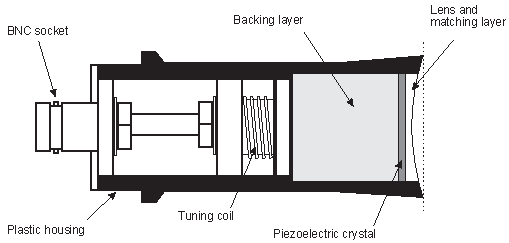
\includegraphics[width=.6\textwidth]{2_transducer_construction-cropped.pdf}
	\caption[Single element ultrasound transducer construction]{Single element ultrasound transducer construction \cite{JensenUltrasoundBook}}
	\label{fig:2_transducer_construction}
\end{figure}

A layperson knows transducers as speakers and microphones in the context of PA systems. In the case of medical \gls{us} it is the device that generates the acoustic pressure field, which is emitted into the tissue. A common type of \gls{us} transducer is a \gls{pzt} type, which has a piezoelectric crystal inside the housing. When excited, this crystal emits ultrasound waves toward flowing blood. The red blood cells will reflect a fraction of the emitted waves. These reflected waves are of a different frequency than the transmitted wave. If the red blood cells move away from the transducer, the frequency will be lower. If the red blood cells are moving towards the transducer, the frequency will be higher. This is caused by the \gls{doppler}. The reflected ultrasonic waves return to the crystal and are converted back into electrical signals. The single-element transducer shown in \cref{fig:2_transducer_construction} has a minimal imaging window and has to be mechanically manipulated to obtain a wide window, which is unfeasible for responsive high-frequency imaging. Thus, usually, a transducer array is used. Various types of \gls{us} transducer exist with different strengths and weaknesses, shown in \cref{fig:2_transducer_types}.

\begin{figure}[htbp]
	\centering
	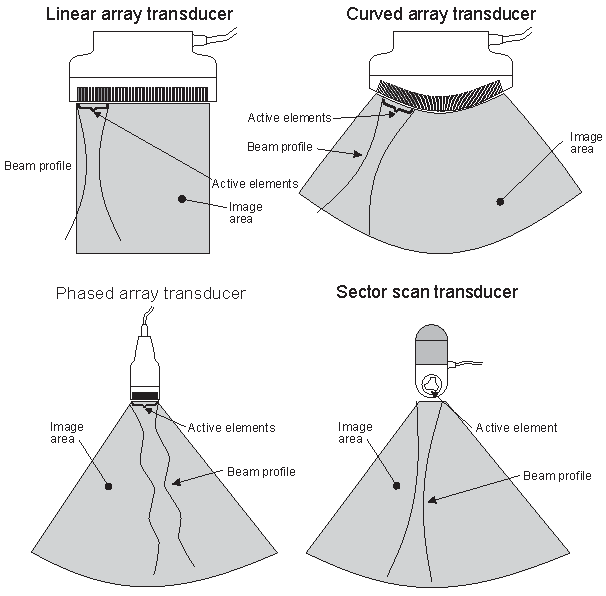
\includegraphics[width=.8\textwidth]{2_transducer_types-cropped.pdf}
	\caption[Transducer types for acquiring B-mode images]{Transducer types for acquiring B-mode images \cite{JensenUltrasoundBook}}
	\label{fig:2_transducer_types}
\end{figure}

\subsection{Doppler effect} \label{sec:doppler_effect}

\begin{figure}[htbp]
	\centering
	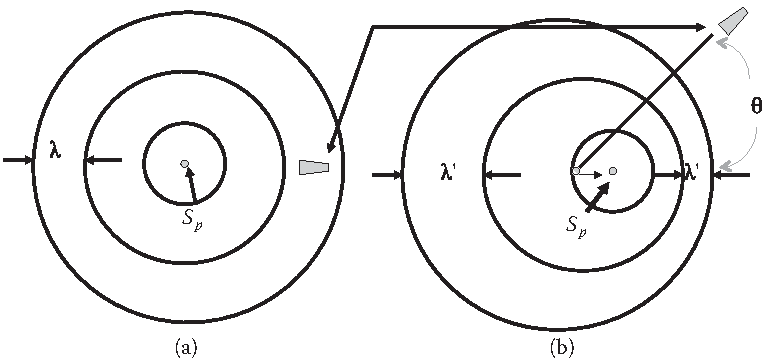
\includegraphics[width=.8\textwidth]{2_doppler_shung-cropped.pdf}
	\caption[Doppler effect diagram]{Doppler effect diagram. A stationary observer perceives a change in the frequency of a wave generated by a moving source toward the observer as a result of a wavelength shift from $\lambda\ $ to $\lambda^{\prime}$. In (a), the source is still. In (b), the source is moving at a velocity $v$. \cite{ShungUltrasound_Book}}
	\label{fig:2_doppler_effect}
\end{figure}

The Doppler effect is a phenomenon in which an observer perceives a shift in the frequency of sound emitted from a source when either the source or the observer is moving, or both are moving. The reason for the perceived change in frequency is visualised in \cref{fig:2_doppler_effect}. In diagram (a), the source $S_{p}$ is stationary and produces a spherical distribution pattern of the wave with the perceived frequency of the observer is given by $f=\sfrac{c}{\lambda}$, where $c$ is the velocity of the wave in the medium and $\lambda$ is the wavelength. In diagram (b), the sound source is moving towards the right with a velocity $v$. The locomotion of the source changes the distribution pattern and causes a longer wavelength on the left, indicating a lower perceived frequency, and a shorter wavelength on the right, indicating a higher perceived frequency, both denoted as $\lambda^{\prime}$ in the diagram. In the case of the observer on the right side, the perceived frequency becomes \cref{eq:2_doppler_effect}.

\begin{equation} \label{eq:2_doppler_effect}
	f^{\prime} = \frac{c}{\lambda} = \frac{c}{\lambda - v T} = \frac{c}{(c-v)T} = \frac{c}{c-v}\cdot f_{0}
\end{equation}

And vice versa, on the left side, the perceived frequency becomes \cref{eq:2_doppler_effect2}.

\begin{equation} \label{eq:2_doppler_effect2}
	f^{\prime} = \frac{c}{c+v} \cdot f_{0}
\end{equation}

This perceived difference between the frequency that is transmitted from the source $f_{0}$, and the perceived frequency $f^{\prime}$ is also called the Doppler frequency, $f_{d}$. When these connections are combined, the Doppler frequency for a source moving with velocity $v$ and an observer travelling with velocity $v^{\prime}$ is given by \cref{eq:2_doppler_moving}.

\begin{equation} \label{eq:2_doppler_moving}
	f_{d} = f^{\prime} - f = \left( \frac{c + v^{\prime}}{c - v}-1 \right)
\end{equation}

If both source and observer are moving with the same velocity, $v$, assuming $c\gg v$, the $v$ cancels out and the expression is reduced to \cref{eq:2_doppler_reduced}.

\begin{equation} \label{eq:2_doppler_reduced}
	f_{d} = \frac{2 v f}{c}
\end{equation}

If the velocity of the moving source is traveling with an incident angle $\theta$, the $v$ in \cref{eq:2_doppler_reduced} is replaced with $v (\cos\theta)$. This results in the expression found in \cref{eq:2_doppler_theta} and forms the basis for applied \gls{doppler} measurements.
\begin{equation} \label{eq:2_doppler_theta}
	\boxed{f_{d} = \frac{2 v(\cos\theta) f}{c}}
\end{equation}

The Doppler effect is used in ultrasonic Doppler devices used to image blood flow \gls{transcutaneous}ly. An ultrasonic transducer in these devices sends ultrasonic waves into a blood artery, and the scattered radiation from moving red cells is measured by either the same transducer or a second transducer. The Doppler frequency, which is determined by the velocity of red blood cells, is extracted using modern electronic demodulation techniques which will be explored later.

\section{Flow Physics}
\begin{figure}[htbp]
	\centering
	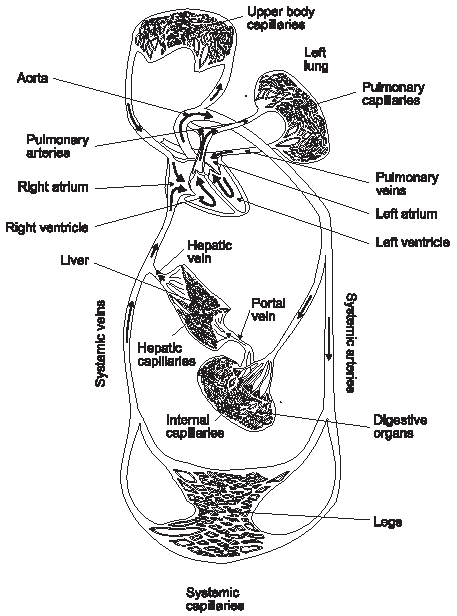
\includegraphics[width=\textwidth]{2_flow_circulatory_system_cropped.pdf}
	\caption[Circulatory system of the human body]{Circulatory system of the human body \cite{JensenUltrasoundBook}}
	\label{fig:2_circulatory_system}
\end{figure}

The flow physics of the human circulatory system are sophisticated, and numerous non-stationary flow patterns are observed. The human circulatory system takes care of transporting oxygen and nutrients to organs, as well as disposing of waste products produced by metabolism. It is possible because the blood within the circulatory system contains several smaller sub-components, such as plasma and formed cellular elements that perform these vital functions. Initially, blood is discharged from the left ventricle of the heart through the aorta and travels to all areas of the body through multiple branches of the arterial tree. When blood flows through the arteries, it enters smaller channels known as arterioles. These arterioles lead to a network of tiny capillaries through which nutrients and waste materials are exchanged between the blood and the organs. The capillaries connect to form a network of venulae, which supply the veins and deliver blood back to the heart. This system, in its entirety, is called systemic circulation. A diagram of the circulatory system as described above can be seen in \cref{fig:2_circulatory_system}. In summary, when examining the elements that comprise the circulatory system, it consists of several components:
\begin{itemize}
	\item Heart, the primary organ of the circulatory system that maintains blood pressure and controls blood velocity.
	\item Blood, and its sub-components
	\begin{itemize}
		\item Plasma, which forms the primary volume, contains nutrients and formed cellular elements.
		\item Red and white blood cells, which carry oxygen and fight off infections, respectively.
		\item Platelets, which are also known as thrombocytes, have the function of clotting during blood vessel injury.
	\end{itemize}
	\item Blood vessels
	\begin{itemize}
		\item Arteries (and arterioles), transport oxygenated blood to organs and tissues at high pressure and velocity.
		\item Capillaries are thin but wide-ranging blood vessels that perform the exchange of matter between the circulatory system and tissue.
		\item Veins (and venulae) carry blood back to the heart at low pressure and velocity.
	\end{itemize}
\end{itemize}

\subsection{Blood flow}
Blood flow is the amount of blood that goes through a blood vessel in a particular period of time, and has a complicated flow pattern due to its pulsing flow. Advanced analysis of haemodynamics is not within the scope of this report, so the explanation will be brief. The primary forces that determine the blood flow $F$ are the pressure difference across a blood vessel and vascular resistance. It is determined by Ohm's law as in \cref{eq:2_flow_ohms_law}.
\begin{equation} \label{eq:2_flow_ohms_law}
	F = \frac{\Delta P}{R}
\end{equation}
Where $\Delta P$ is the pressure difference across the blood vessel and $R$ is the vascular resistance. The pressure difference $\Delta P$ is calculated with \cref{eq:2_pressure_diff}.
\begin{equation} \label{eq:2_pressure_diff}
	\Delta P = P_{1}-P_{2}
\end{equation}
Where $P_{1}$ and $P_{2}$ are the blood pressures measured at each end of the blood vessel. Pressure has significant importance on blood flow because an increase in arterial pressure not only increases the force that pushes blood through the capillaries but also expands the vessels, lowering vascular resistance. Selected dimensions and flow characteristics can be seen in \cref{tab:2_dimensions_flow_vessels}.

\begin{table}[htbp]
	\centering
	\caption[Typical dimensions and flow in human circulatory system]{Typical dimensions and flow in human circulatory system \cite{JensenUltrasoundBook}}
	\begin{adjustbox}{max width=\textwidth}
		\label{tab:2_dimensions_flow_vessels}
		\sisetup{range-phrase=--,range-exponents = combine}
		\begin{tblr}[]{%
				width=\textwidth,
				%width=.9\textwidth,
				colspec = {lSSSSSSSS
				},
				row{1} = {guard, m, font=\small\bfseries},
				%vlines, hlines,
			}
			\toprule
			Vessel & {Internal\\diameter\\(\unit{\centi\meter})} & {Wall\\thickness\\(\unit{\centi\meter)}} & {Length\\(\unit{\centi\meter})} & {Young's\\modulus\\(\unit{\newton\per\meter\squared\cdot10^{5})}} & {Peak\\velocity\\(\unit{\centi\meter\per\second})} & {Mean\\velocity\\(\unit{\centi\meter\per\second})} & {Reynolds\\number\\(\unit{\mathrm{peak}})} & {Pulse\\propagation\\velocity\\(\unit{\centi\meter\per\second})}	\\
			\midrule
			Ascending aorta & \numrange{1}{2.4} & \numrange{0.05}{0.08} & 5 & \numrange{3}{6} & \numrange{20}{290} & \numrange{10}{40} & 4500 & \numrange{400}{600}	\\
			Descending aorta & \numrange{0.8}{1.8} & \numrange{0.05}{0.08} & 20 & \numrange{3}{6} & \numrange{25}{250} & \numrange{10}{40} & 3400 & \numrange{400}{600} \\
			Abdominal aorta & \numrange{0.5}{1.2} & \numrange{0.04}{0.06} & 15 & \numrange{9}{11} & \numrange{50}{60} & \numrange{8}{20} & 1250 & \numrange{600}{700}\\
			Femoral artery & \numrange{0.2}{0.8} & \numrange{0.02}{0.06} & 10 & \numrange{9}{12} & \numrange{100}{120} & \numrange{10}{15} & 1000 & \numrange{800}{1030} \\
			Carotid artery & \numrange{0.2}{0.8} & \numrange{0.02}{0.04} & \numrange{10}{20} & \numrange{7}{11} & &  &  & \numrange{600}{1100}\\
			Arteriole & \numrange{0.001}{0.008} & 0.002 & \numrange{0.1}{0.2} &  & \numrange{0.5}{1} &  & 0.09 &  \\
			Capillary & \numrange{0.0004}{0.0008} & 0.0001 & \numrange{0.02}{0.1} &  & \numrange{0.02}{0.17} &  & 0.001 &  \\
			Inferior vena cava & \numrange{0.6}{1.5} & \numrange{0.01}{0.02} & \numrange{20}{40} & \numrange{0.4}{1} & \numrange{15}{40} &  & 700 & \numrange{100}{700}\\
			\bottomrule
		\end{tblr}
	\end{adjustbox}
\end{table}

\section{Transducer}
Various \gls{transducer} types are used during the testing of this project. Initially, commercially available transducers were used in order to validate the experimental process of the pulse-echo and Doppler measurements. Commercially available transducers in this context mean \gls{pzt} \gls{piezoelectric} transducers. PZT is a piezoelectric material that deforms when an electrical voltage is applied and generates an electrical signal when it is mechanically deformed. PZT transducers are widely used for medical imaging due to their high piezoelectric efficiency, high bandwidth and durability.

At a later stage during the project, CMUTs are used. CMUT, is a newer technology that uses capacitance to convert between electrical and mechanical energy. The transducer consists of a flexible membrane that moves in response to an applied voltage, producing ultrasound signals. CMUTs have advantages in terms of their small size, high frequency, and ability to operate in a broad range of conditions, making them ideal for use in portable and high-resolution imaging devices. They can be produced in large quantities using micro-machining processes that ensure tight parameter specifications, which is difficult to achieve with piezoelectric transducers. Fabricating CMUTs is also simpler than piezoelectric transducers, and batch processing allows for the creation of transducer arrays with various geometries and operating frequencies on a single wafer. The use of standard IC processes also makes it convenient to integrate CMUT arrays with supporting electronics. Additionally, CMUTs can operate over a wider temperature range than piezoelectric devices. Over the last decade, results have demonstrated that CMUTs optimized with regard to design parameters such as device size, membrane radius, thickness, shape, gap height, and operating mode can compare favourably to piezoelectric transducers in terms of bandwidth (\qty{170}{\percent}), frequency range (\qtyrange[scientific-notation = engineering]{0.1}{70}{\mega\hertz}) \todo{Ret til med korrekt enhed}, dynamic range (\qty{130}{\decibel\per\volt}), maximum output pressure (\qty{35}{\kilo\pascal\per\volt}), and receive sensitivity (\qty{50}{\decibel\per\pascal\per\hertz}). There are two types of CMUTs used:

\subsubsection{Rigid CMUTs:}
\begin{itemize}
	\item Advantages:
	\begin{itemize}
		\item Higher mechanical stability, leading to less noise and improved image quality
		\item Can handle higher pressures, making them suitable for deeper imaging applications
		\item Can have a larger surface area, providing higher sensitivity
	\end{itemize}
	\item Disadvantages:
	\begin{itemize}
		\item Less flexible, limiting their use in applications with complex geometries or limited access
		\item Higher stiffness, leading to increased power consumption and difficulty in producing high-frequency signals
	\end{itemize}
\end{itemize}
\subsubsection{Flexible CMUTs:}
\begin{itemize}
	\item Advantages:
	\begin{itemize}
		\item More flexible, allowing them to conform to complex geometries or be used in applications with limited access
		\item Can be made thinner and lighter, making them suitable for portable or handheld imaging devices
		\item Can be integrated into wearable devices or implanted into the body, enabling new imaging modalities
	\end{itemize}
	\item Disadvantages:
	\begin{itemize}
		\item Lower mechanical stability, leading to increased noise and reduced image quality
		\item Lower maximum operating pressure, limiting their use in deep imaging applications
		\item Smaller surface area, resulting in reduced sensitivity
	\end{itemize}
\end{itemize}
In summary, the choice between rigid and flexible CMUTs depends on the specific requirements of the application and the trade-off between flexibility, sensitivity, and image quality. For this project, a wearable transducer is desired and therefore the flexible CMUT is preferred.

\subsubsection{Structure}
\begin{figure}[htbp]
	\centering
	%		

\tikzset{every picture/.style={line width=0.75pt}} %set default line width to 0.75pt

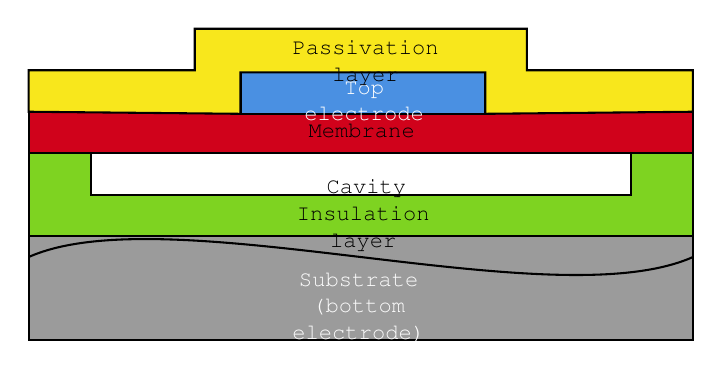
\begin{tikzpicture}[x=0.75pt,y=0.75pt,yscale=-1,xscale=1]
	%uncomment if require: \path (0,171); %set diagram left start at 0, and has height of 171

	%Shape: Rectangle [id:dp9408379535361424]
	\draw  [fill={rgb, 255:red, 155; green, 155; blue, 155 }  ,fill opacity=1 ] (10,110) -- (330,110) -- (330,160) -- (10,160) -- cycle ;
	%Curve Lines [id:da14073546290370997]
	\draw    (10,120) .. controls (77.23,90) and (262.77,150) .. (330,120) ;
	%Shape: Polygon [id:ds29154118264594087]
	\draw  [fill={rgb, 255:red, 126; green, 211; blue, 33 }  ,fill opacity=1 ] (330,70) -- (330,110) -- (10,110) -- (10,70) -- (40,70) -- (40,90) -- (300,90) -- (300,70) -- cycle ;
	%Shape: Rectangle [id:dp7293209428281849]
	\draw  [fill={rgb, 255:red, 208; green, 2; blue, 27 }  ,fill opacity=1 ] (10,50) -- (330,50) -- (330,70) -- (10,70) -- cycle ;
	%Shape: Rectangle [id:dp8584212117739504]
	\draw  [fill={rgb, 255:red, 74; green, 144; blue, 226 }  ,fill opacity=1 ] (112.05,31) -- (229.95,31) -- (229.95,51) -- (112.05,51) -- cycle ;
	%Shape: Polygon [id:ds9961529541546873]
	\draw  [fill={rgb, 255:red, 248; green, 231; blue, 28 }  ,fill opacity=1 ] (10,30) -- (10,50) -- (112.05,51) -- (112.05,31) -- (229.95,31) -- (229.95,51) -- (330,50) -- (330,30) -- (250,30) -- (250,10) -- (90,10) -- (90,30) -- cycle ;

	% Text Node
	\draw (136,34) node [anchor=north west][inner sep=0.75pt]  [font=\footnotesize,color={rgb, 255:red, 255; green, 255; blue, 255 }  ,opacity=1 ] [align=left] {\begin{minipage}[lt]{51.23pt}\setlength\topsep{0pt}
			\begin{center}
				{\fontfamily{pcr}\selectfont Top electrode}
			\end{center}

	\end{minipage}};
	% Text Node
	\draw (142,54) node [anchor=north west][inner sep=0.75pt]  [font=\footnotesize] [align=left] {\begin{minipage}[lt]{40.37pt}\setlength\topsep{0pt}
			\begin{center}
				{\fontfamily{pcr}\selectfont Membrane}
			\end{center}

	\end{minipage}};
	% Text Node
	\draw (131,94) node [anchor=north west][inner sep=0.75pt]  [font=\footnotesize] [align=left] {\begin{minipage}[lt]{58.04pt}\setlength\topsep{0pt}
			\begin{center}
				{\fontfamily{pcr}\selectfont Insulation layer}
			\end{center}

	\end{minipage}};
	% Text Node
	\draw (152,75) node [anchor=north west][inner sep=0.75pt]  [font=\footnotesize] [align=left] {\begin{minipage}[lt]{26.25pt}\setlength\topsep{0pt}
			\begin{center}
				{\fontfamily{pcr}\selectfont Cavity}
			\end{center}

	\end{minipage}};
	% Text Node
	\draw (121,126) node [anchor=north west][inner sep=0.75pt]  [font=\footnotesize] [align=left] {\begin{minipage}[lt]{69.77pt}\setlength\topsep{0pt}
			\begin{center}
				{\fontfamily{pcr}\selectfont \textcolor[rgb]{0.99,0.99,0.99}{Substrate}}\\{\fontfamily{pcr}\selectfont \textcolor[rgb]{0.99,0.99,0.99}{(bottom electrode)}}
			\end{center}

	\end{minipage}};
	% Text Node
	\draw (129,14) node [anchor=north west][inner sep=0.75pt]  [font=\footnotesize] [align=left] {\begin{minipage}[lt]{62.71pt}\setlength\topsep{0pt}
			\begin{center}
				{\fontfamily{pcr}\selectfont Passivation layer}
			\end{center}

	\end{minipage}};


\end{tikzpicture}

	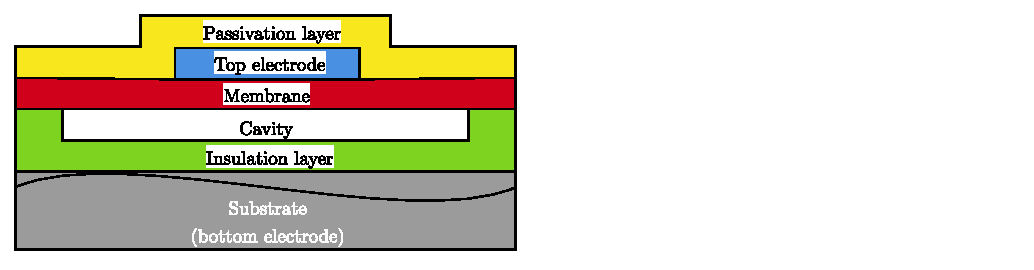
\includegraphics[width=.6\textwidth]{Figures/3_cmut_structure.pdf}
	\caption{Basic CMUT structure}
	\label{fig:3_cmut_structure}
\end{figure}
The key components of the structure are the cavity, membrane, and electrode. CMUT transducers are fabricated using standard \gls{ic} fabrication processes, resulting in a capacitor cell that consists of a metallized membrane (top electrode) suspended above a heavily doped silicon substrate (bottom electrode), as depicted in \cref{fig:3_cmut_structure}. An insulating layer is included to prevent the two electrodes from making contact and shorting. A single transducer element consists of multiple small capacitor cells connected in parallel. By arranging transducer elements in various geometries, any array shape can be achieved, as demonstrated in \cref{fig:3_cmut_array_shape}. In (a), circular membranes with a diameter of \qty{24}{\micro\meter} have approximately \qty{50}{\percent} active area coverage. In (b), circular membranes with a diameter of \qty{80}{\micro\meter} have \qty{72}{\percent} active area coverage. (c) displays hexagonal membranes with a diameter of \qty{80}{\micro\meter} that have \qty{86}{\percent} active area coverage. Finally, (d) demonstrates tented membranes in which the etch holes are located on the post, providing over \qty{90}{\percent} active area coverage.

\begin{figure}[htbp]
	\centering
	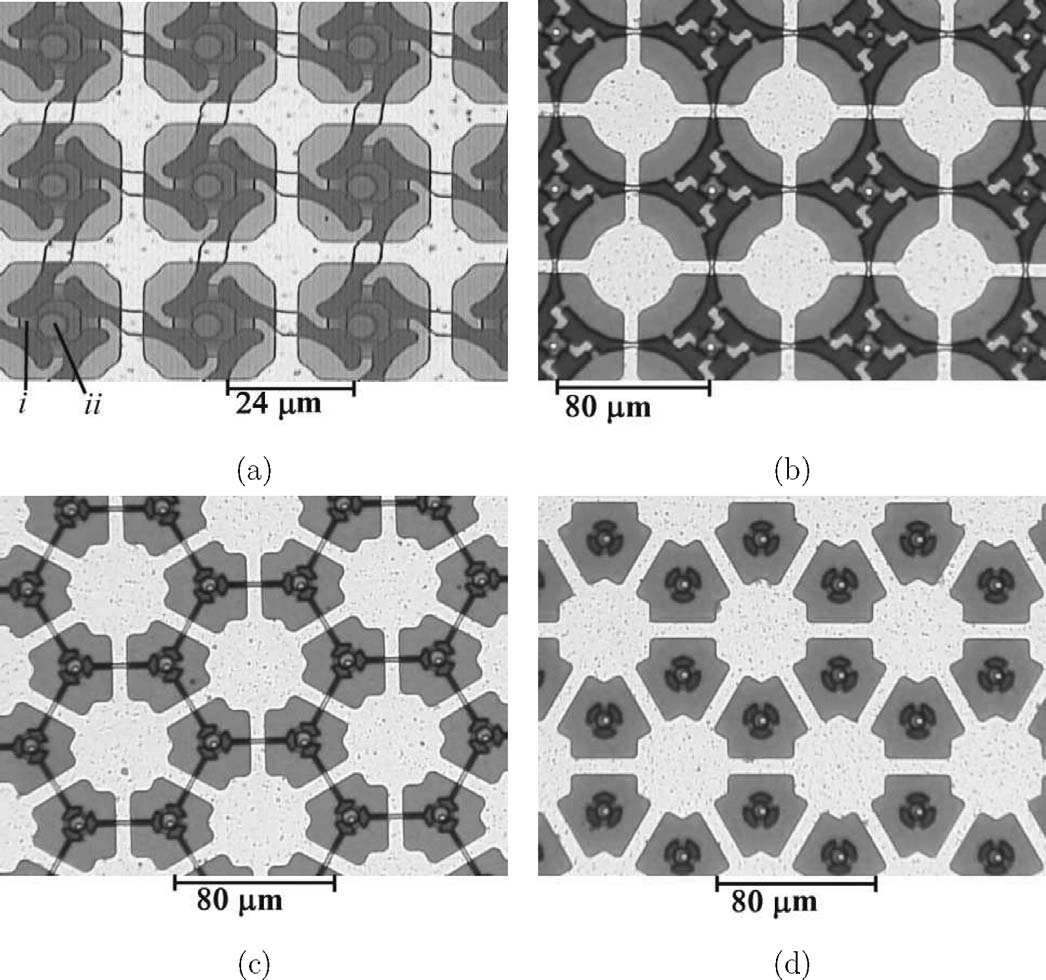
\includegraphics[width=.6\textwidth]{Figures/3_cmut_array_shapes.jpg}
	\caption[Optical images of various cMUT elements with different membrane shapes]{Optical images of various cMUT elements with different membrane shapes and sizes are shown to illustrate their relationship to active area coverage \cite{cmut_array_shape}}
	\label{fig:3_cmut_array_shape}
\end{figure}

%\subsection{Impedance matching}
%Impedance matching refers to the adjustment of the output impedance of the transducer to match the input impedance of the receiving system, such as the ultrasound machine or amplifier. This ensures maximum transfer of energy from the transducer to the receiving system, leading to improved signal strength and reduced noise in the final image. In ultrasound imaging, the transducer is used to both transmit and receive ultrasound signals. The impedance of the transducer must be carefully matched to the environment it is operating in, to ensure efficient transfer of energy both ways. If the impedance of the transducer and the receiving system does not match, a portion of the transmitted energy will be reflected back to the transducer, leading to reduced signal strength and increased noise in the final image. This can also result in increased power consumption and reduced battery life in portable or handheld imaging devices.

\section{Devices}
\begin{figure}[htbp]
	\centering
	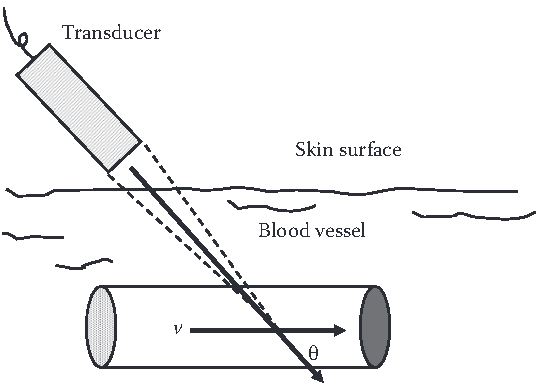
\includegraphics[width=.6\textwidth]{2_ultrasound_scan.pdf}
	\caption[Diagram of ultrasound wave transmitted and reaching blood vessel with incident angle $\theta$]{Diagram of \gls{us} wave transmitted and reaching blood vessel with incident angle $\theta$ \cite{ShungUltrasound_Book}}
	\label{fig:2_ultrasound_flow_scan}
\end{figure}

A device that measures the flowing of blood is called a flowmeter. Flowmeters may be used both inside and outside of vessels. One of the flowmeters that may be used outside the vessel to monitor flow is \gls{us}. \Cref{fig:2_ultrasound_flow_scan} depicts an ultrasonic wave of frequency $f$ insonifying a blood artery, resulting in an angle of $\theta$ relative to velocity $v$. For simplicity, it is assumed that blood flows in a vessel at a constant velocity $v$. The echoes returned are shifted in frequency as described in \cref{eq:2_doppler_theta} earlier in the chapter. The echoes scattered by blood after being insonified by an ultrasonic wave convey information about the velocity of blood flow. Blood flow measurements are often used in clinical settings to determine the status of blood vessels and organ functioning. The two commonly used fundamental techniques for ultrasound Doppler flow measurements are \gls{cw} and \gls{pw}. Both will be explained.

\subsection{Continuous-wave Flowmeter}
\begin{figure}[htbp]
	\centering
	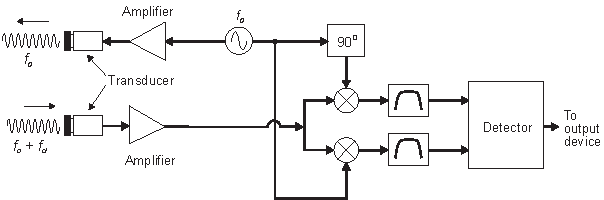
\includegraphics[width=\textwidth]{2_blockdiagram_cwdoppler.pdf}
	\caption[Block diagram of continuous-wave flowmeter]{Block diagram of \gls{cw} flowmeter \cite{JensenUltrasoundBook}}
	\label{fig:2_devices_cw}
\end{figure}
The earliest non-invasive cardiovascular diagnostic technologies relied heavily on \gls{cw} Doppler flowmeters. To continuously transmit waves and receive signals from moving reflectors, the \gls{cw} flowmeter uses two transducers. \gls{cw} flowmeters use less sophisticated electronics than \gls{pw} flowmeters. A drawback to the \gls{cw} flowmeter is the lacking depth discrimination due to the continuous characteristic of this device type. A block diagram of a typical \gls{cw} flowmeter can be seen in \cref{fig:2_devices_cw}. The basic principles of the device are previously explained in \cref{sec:doppler_effect}, and the measurement of the device is described in \cref{eq:2_doppler_effect}. The device continuously emits an ultrasonic wave in the first transducer expressed as a function of time by \cref{eq:2_cw_tx} \cite{JensenUltrasoundBook}.
\begin{equation} \label{eq:2_cw_tx}
	e(t) = \cos (2\pi f_{0} t)
\end{equation}
While receiving the backscattered signal on the second transducer expressed by \cref{eq:2_cw_rx} \cite{JensenUltrasoundBook}.
\begin{align} \label{eq:2_cw_rx}
	r_{s}(t) &= a \cos \left( 2\pi f_{0} \alpha (t-t_{0}) \right) \\
	\alpha &\approx 1 - \frac{2 v_{z}}{c} \\
	\alpha t_{0} &\approx \frac{2 d_{0}}{c}
\end{align}
Where $v_{z}$ indicates the velocity in the $z$ direction. Applying the Fourier transform, the expression yields \cref{eq:2_cw_fourier}.
\begin{equation} \label{eq:2_cw_fourier}
	r_{s}(t)\cdot e^{j2\pi f_{0} t} \Longleftrightarrow R_{s}(f-f_{0})
\end{equation}
Where $R_{s}(f-f_{0})$ is the Fourier transform of $r_{s}(t)$. The received signal is then multiplied with a quadrature signal of frequency $f_{0}$ to find the Doppler frequency in \cref{eq:2_cw_quadrature}.
\begin{align} \label{eq:2_cw_quadrature}
	m(t) &= a \left[ \cos(2\pi f_{0} t) + j\sin (2\pi f_{0} t) \right] \cos (2\pi f_{0} \alpha (t-t_{0})) \\
	&= \frac{a}{2} \Bigl\{ \cos (2\pi f_{0} [ (1-\alpha) t- \alpha t_{0} ]) + \cos (2\pi f_{0} [ (1-\alpha) t- \alpha t_{0} ]) \\
	&\quad + j \sin (2\pi f_{0} [ (1-\alpha) t- \alpha t_{0} ]) + j \sin (2\pi f_{0} [(1-\alpha) t- \alpha t_{0} ]) \Bigr\} \nonumber
\end{align}

As is general for quadrature demodulation, the resulting signal contains the frequency components of the sum and difference of the emitted and received signals' frequencies shown in \cref{fig:2_demod_fd_frequency_domain}, where the signals are shown in time and frequency domains.

\begin{figure}[htbp]
	\centering
	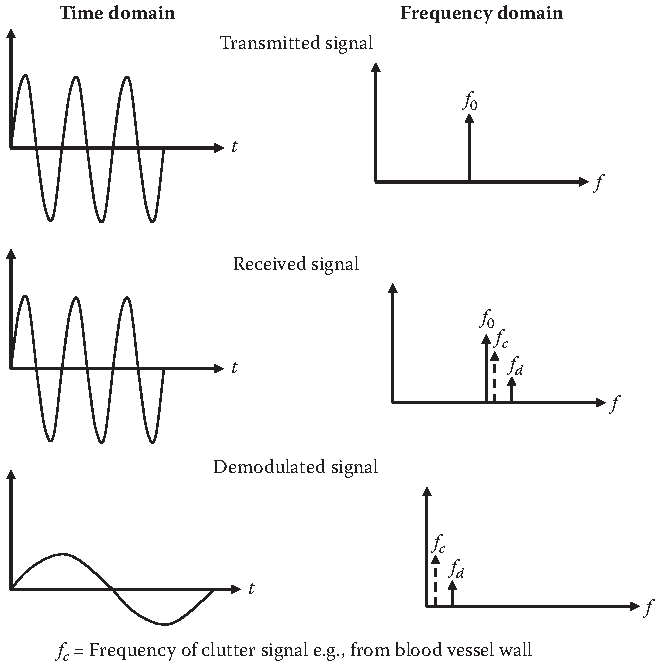
\includegraphics[width=.8\textwidth]{2_demod_fd_frequency_domain-cropped.pdf}
	\caption[Demodulation effects of Doppler signals in time and frequency domain]{Demodulation effects of Doppler signals in time and frequency domain \cite{ShungUltrasound_Book}}
	\label{fig:2_demod_fd_frequency_domain}
\end{figure}

Generally, a \gls{bp} filter is used on the demodulated signal to remove the high-frequency summed signal at twice the frequency of $f_{0}$. The filtered signal after the \gls{bp} filter is expressed by \cref{eq:2_cw_bp} and contains the Doppler shift of the emitted signal.
\begin{equation} \label{eq:2_cw_bp}
	m_{f}(t) \approx \frac{a}{2} e^{\left(j2\pi f_{0} \frac{2v_{z}}{c}t\right)} e^{\left( -j2\pi f_{0} \alpha t_{0} \right)}
\end{equation}
Where the second exponential term is the delay proportional to the time between transmission and receiving of the signal. The selected cutoff frequency is chosen to be much lower than the carrier frequency to remove the carrier wave. One issue with ultrasonic Doppler blood flow monitoring is that the blood vessels that generate large reflected echoes are also moving with a low velocity. These big, slow-moving echoes are referred to as clutter signals in Doppler nomenclature. The band pass filter's low-end cutoff frequency must be designed to minimize interference from these clutter signals. The design of this band pass filter in the low-frequency region, which serves the function of high pass, also known as a clutter rejection filter, has proven troublesome since the magnitude of clutter signals is many orders greater than that of blood and may obfuscate those from slow-moving blood.

\begin{table}[htbp]
	\centering
	\caption[Measured frequency shifts with a Doppler \qty{3}{\mega\hertz} transducer at various velocities at a \qty{45}{\degree} incident angle]{Measured frequency shifts with a Doppler \qty{3}{\mega\hertz} transducer at various velocities at a \qty{45}{\degree} incident angle \cite{JensenUltrasoundBook}}
	\label{tab:2_cw_frequency_shifts}
	\begin{tblr}[]{%
			colspec = {SS},
			row{1} = {guard, m, font=\small\bfseries},
			%vlines, hlines,
		}
		\toprule
		{Velocity $\left(v\right)$ \\ \unit[per-mode = symbol]{\meter\per\second}} & {Doppler frequency $\left(f_{d}\right)$ \\ \unit{\hertz} } \\
		\midrule
		0.01 & 28 \\
		0.1 & 276 \\
		0.5 & 1377 \\
		1 & 2755 \\
		2 & 5510 \\
		5 & 13770 \\
		\bottomrule
	\end{tblr}
\end{table}

Seen in \cref{tab:2_cw_frequency_shifts} is an example of measured Doppler frequencies using a \qty{3}{\mega\hertz} transducer using the method shown in \cref{fig:2_ultrasound_flow_scan}. Note that the measured frequencies are all within the audible range.

\subsection{Pulsed-wave Flowmeter}
\begin{figure}[htbp]
	\centering
	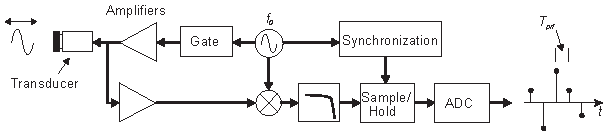
\includegraphics[width=\textwidth]{2_blockdiagram_pwdoppler.pdf}
	\caption[Block diagram of pulsed-wave flowmeter]{Block diagram of \gls{pw} flowmeter \cite{JensenUltrasoundBook}}
	\label{fig:2_devices_pw}
\end{figure}
The concept of a pulsed-wave flowmeter was proposed in \cite{Baker1970} and other related articles. This type of flowmeter is periodically changing from a transmitter to a receiver. In the transmit mode, the transducer emits a series of pulses. When in the receiving mode, the transducer is listening for the backscattered signal. A simplified block diagram can be seen in \cref{fig:2_devices_pw}. The movement of particles within the blood causes a displacement in the backscattered signal. These systems are commonly referred to as \enquote{Doppler systems} even though it is somewhat misleading. The effects of attenuation are also causing a shift in frequency of a higher magnitude than the velocity of particles in the blood. This is because the conventional Doppler effect is not the straightforward methodology that is applied to the analysis of the back-scattered signal. It is, in fact, an artefact. It is the shift in the location of the scatters that is observed, not the shift in the transmitted frequency. \Cref{fig:2_pw_sampling_displacement} shows the received signal after demodulation and filtering; the depth in tissue is fixed here, and the signals displayed on the left side of the figure are the result of a pulse sequence. Each line represents a single pulse, and each pulse is emitted at a pulse repetition frequency, $f_{\mathrm{prf}}$. Instead, on the right, the dotted line shows the sampled signal formed by taking into account the amplitude of each pulse after a specified time period. To depict the signals on the graph, a single pulse is emitted for each line, and the signals are displaced in amplitude. The sampled signal is displayed on the right.
\begin{figure}[ht]
	\centering
	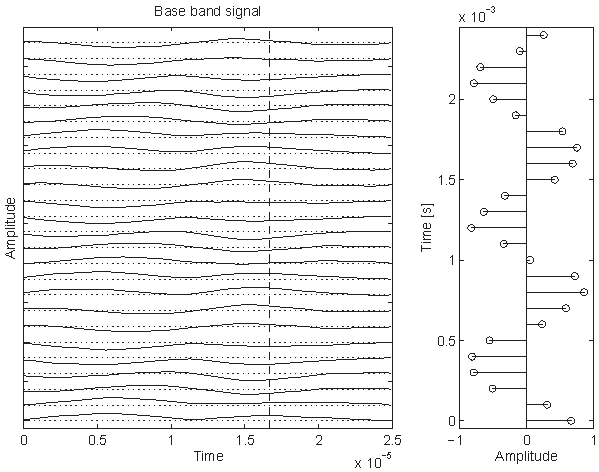
\includegraphics[width=.8\textwidth]{2_pw_pulse_sampling_displacement.pdf}
	\caption[Sampling for a gate pulsed wave system with a single range]{Sampling for a gate pulsed wave system with a single range \cite{JensenUltrasoundBook}}
	\label{fig:2_pw_sampling_displacement}
\end{figure}
In the pulsed-wave flowmeter, the received signal is described by \cref{eq:2_pw_receive_signal_a,eq:2_pw_receive_signal_b,eq:2_pw_receive_signal_c,eq:2_pw_receive_signal_d} \cite{JensenUltrasoundBook}.
\begin{subequations}
	\begin{align}
		r_{s}(t) &= a\cdot e^{\left( \alpha \left( t-t_{0} \right) \right)} \label{eq:2_pw_receive_signal_a} \\
		\alpha &= \left( 1- \frac{2v_{z}}{c} \right) \label{eq:2_pw_receive_signal_b} \\
		\alpha t_{0} &= \frac{2d_{0}}{c} \label{eq:2_pw_receive_signal_c} \\
		v_{z} &= \left| \vec{v} \right| \cos \theta \label{eq:2_pw_receive_signal_d}
	\end{align}
\end{subequations}
\Cref{eq:2_pw_ts_time_shift} provides the calculation for the time shift $t_{s}$ of the RF signal between two emissions, which is determined by the distance that the scatterer moves in the direction of the ultrasound beam proportional to the velocity component $v_{z}$.
\begin{equation} \label{eq:2_pw_ts_time_shift}
	t_{s} = \frac{2v_{z}}{c} T_{\mathrm{prf}}
\end{equation}
Where $c$ is the speed of sound in the medium, $T_{\mathrm{prf}}$ is the interval between each pulse emission. To measure the movement of the scatterer, the signal can be recorded at a certain depth. By selecting one sample at that specific depth for each line, a sampled signal with a frequency that corresponds to the scatter velocity can be obtained. Hypothetically, if the velocity of stationary scatterers in blood was measured, a constant amplitude would be measured. A change in the sample value is observed when there is movement. Between two pulses, the scatterer movement is proportional to the velocity $v_{z}$ in the direction of the ultrasound beam. Taking one sample from each line at a certain depth yields a sampled signal with a frequency proportional to the scatter velocity. After the back-scattered signal is received it is multiplied by the centre frequency of the emitted pulse and filtered to remove the sum frequency \cite{JensenUltrasoundBook}. A \gls{adc} quantifies the signal for further signal processing. Referring to displacement \cref{fig:2_pw_sampling_displacement} again, the dashed vertical line represents the sample of each pulse that is taken. If sampling is done $T_{s}$ after pulse emission, the measurement depth is expressed by \cref{eq:2_pw_depth}.
\begin{equation} \label{eq:2_pw_depth}
	d_{0} = \frac{T_{s}c}{2}
\end{equation}
Thus, if a sample is taken at the same depth for each line, resulting in a sinusoidal signal proportional in frequency to the scatter velocity \cite{Munk_Thesis}. This technique improved the accuracy of the investigations of blood vessels and facilitated the display of velocity profiles. \Cref{eq:2_pw_receive_signal_i} describes the relationship between the received sampled signal for a single scatter and the sinusoidal pulse emitted by the transducer during the $i\textsuperscript{th}$ pulse emission.
\begin{subequations}
	\begin{align}
		r(i) &= a(i) \sin \left( 2\pi f_{p}i T_{\mathrm{prf}} +\theta \right) \label{eq:2_pw_receive_signal_i} \\
		f_{p} &= \frac{2v_{z}}{c}f_{0} \label{eq:2_pw_receive_signal_fp}
	\end{align}
\end{subequations}
Where $f_{p}$ is expressed by \cref{eq:2_pw_receive_signal_fp}, $a(i)$ is the amplitude for the $i\textsuperscript{th}$ pulse, $f_{0}$ is the emitted frequency, and $\theta$ is the phase factor proportional to the depth of interest.
\section{Blood Velocity Estimation}
\todo{Separer CW og PW estimation}
This section will explain the methodology of velocity estimation, assuming a pulsed-wave system signal is obtained from a back-scattered signal. There are variations of methods that can be applied, but only the implementation that will be used is discussed in this report.

\subsection{Spectral Envelope}
\begin{figure}[htbp]
	\centering
	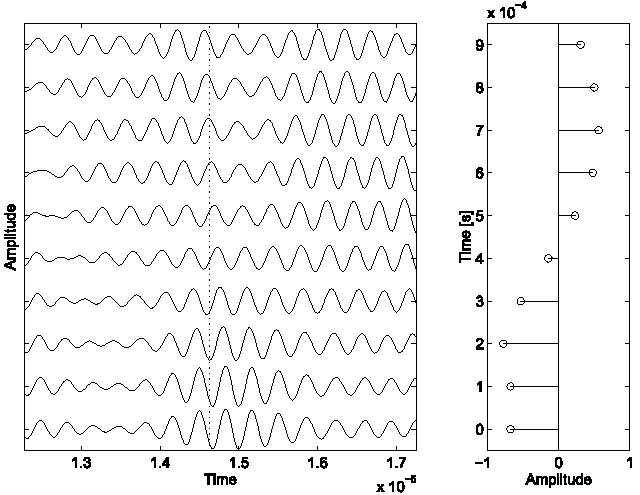
\includegraphics[width=.8\textwidth]{Pictures/./../Figures/2_rf_sampling_simulated.pdf}
	\caption[Simulated RF sampling of a blood vessel]{Simulated RF sampling of a blood vessel with segmented receiver line with a sample interval denoted by a dotted line (left) and the resulting amplitude of the sample (right) \cite{JensenUltrasoundBook}}
	\label{fig:2_rf_sampling_simulated}
\end{figure}
\Cref{fig:2_rf_sampling_simulated} displays a signal where the scatterers in the sampled depth $d_{0}$ move away from the transducer, and the shift in the pulsed signal is present. The measurement is created by taking one sample at a specific depth ($d_0$) for each RF line. The sampling is performed at a frequency of $f_{\mathrm{prf}}$, as indicated by the dotted line in the figure. Due to the slow movement of the received signals past the sample volume, there is a gradual change in the sampled signal over time. As a result of the slow movement of the signals, the frequency of the sampled signal is much lower than that of the RF signal. It's worth noting that the received signal not only shifts in time from pulse to pulse, but its shape also changes. This is because the signal is constructed by adding up responses from many scatterers that move at different speeds. A stationary structure will result in an identical sample value for all segmented RF lines. The spectrum of this stationary signal is shown in \cref{eq:2_stationary_rf_spectrum}.

\begin{equation} \label{eq:2_stationary_rf_spectrum}
	\abs{H_{s}(f)} = \abs{a \frac{\sin (\pi f N T_{\mathrm{prf}})}{\sin (\pi f T_{\mathrm{prf}})}}
\end{equation}
which for $f = 0$ is equal to $aN$ and has its first zero at $\sfrac{f_{\mathrm{prf}}}{N}$. The signal spectrum based on \cref{eq:2_stationary_rf_spectrum} is shown in \cref{fig:2_rf_spectrum_stationary}.

\begin{figure}[htbp]
	\centering
	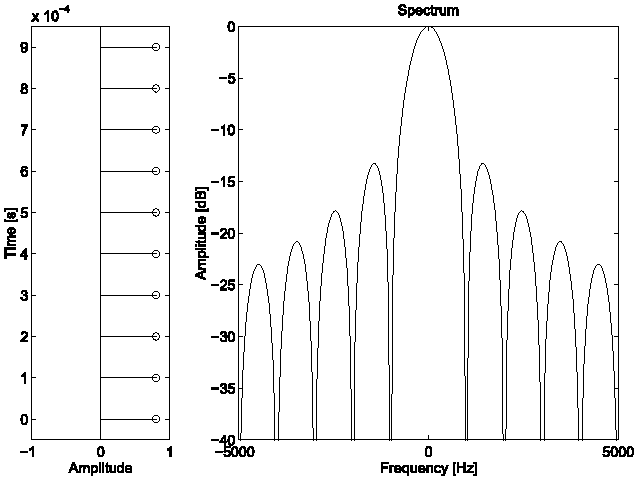
\includegraphics[width=.8\textwidth]{Figures/2_rf_spectrum_stationary.pdf}
	\caption[Stationary tissue sampled signal and stationary tissue sample spectrum]{Stationary tissue sampled signal (left) and stationary tissue sample spectrum (right) \cite{JensenUltrasoundBook}}
	\label{fig:2_rf_spectrum_stationary}
\end{figure}

When dealing with small blood vessels, the stationary echoes can be significantly stronger (up to \qty{40}{\decibel}) than the blood signal itself. To properly visualize blood flow details, the stationary signal must be eliminated from the sonogram. This requires setting the cutoff frequency to at least $f_{\mathrm{prf}} = N$, in order to remove the main component. In some cases, a higher cutoff frequency may be necessary, particularly if the stationary echo is strong or the vessel wall is in motion. The speed and pulse repetition frequency of a single moving scatterer affects the signal received. The signal will look like the pulse, but its time scale and frequency will differ from the RF pulse because the pulse waveform slowly moves past the point where it is measured. \Cref{fig:2_estimation_single_scatterer} shows this, where a beam from a concave transducer is crossed by a single scatterer. The time shift between each line is determined by the expression in \cref{eq:2_estimation_time_shift}.
\begin{figure}[htbp]
	\centering
	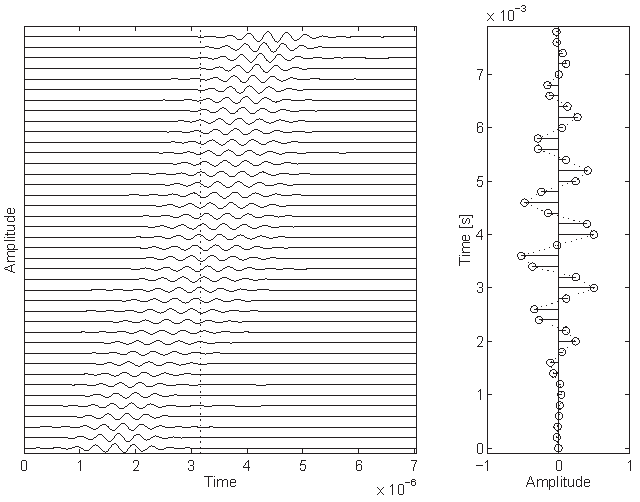
\includegraphics[width=.8\textwidth]{Figures/2_estimation_single_scatterer.pdf}
	\caption[Single moving scatterer crossing a concave transducer beam]{Single moving scatterer crossing a concave transducer beam \cite{JensenUltrasoundBook}}
	\label{fig:2_estimation_single_scatterer}
\end{figure}
\begin{equation} \label{eq:2_estimation_time_shift}
	t_{s} = \frac{2v_{z}}{c} \cdot T_{\mathrm{prf}}
\end{equation}
Which increases linearly by line $i$. Individual sinusoidal components are expressed by \cref{eq:2_estimation_sine_component}.
\begin{equation} \label{eq:2_estimation_sine_component}
	y(i) = \sin \left( 2\pi \frac{2v_{z}}{c}\cdot f_{0} iT_{\mathrm{prf}} \right)
\end{equation}
Where the variable $iT_{\mathrm{prf}}$ corresponds to time and $f_{0}$ corresponds to the fundamental frequency. The received signal frequency is expressed by $\sfrac{2v_{z}}{c}\cdot f_{0}$, where the frequency axis is scaled by factor $\sfrac{2v_{z}}{c}$ as seen in \cref{fig:2_estimation_scaling_axis}. The center frequency transforms to $f_{p} = \frac{2v_{z}}{c} f_{0}$. Every other spectral element is transformed by factor $\frac{2v_{z}}{c}$ and the received signal has the shape of a scaled frequency pulse.
\begin{figure}[htbp]
	\centering
	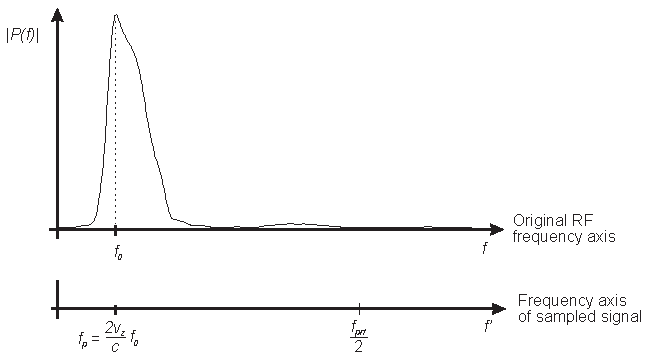
\includegraphics[width=.8\textwidth]{Figures/2_estimation_frequency_scaling.pdf}
	\caption[Frequency axis scaling for scatterer with velocity $v_{z}$]{Frequency axis scaling for scatterer with velocity $v_{z}$ \cite{JensenUltrasoundBook}}
	\label{fig:2_estimation_scaling_axis}
\end{figure}
A sufficient number of lines must be captured, or only a part of the pulse is obtained. In practical terms, it corresponds to weighing the pulse with a rectangular window, which broadens the spectrum. The spectrum of the window is expressed by \cref{eq:2_estimation_spectrum_window} and is convolved\todo{Convolved? Or convoluted?} with the spectrum of the pulse. A narrow spectrum is seen for slow velocities and the resulting spectrum is nearly determined solely by the spectrum of the window.
\begin{equation} \label{eq:2_estimation_spectrum_window}
	W(f) = \frac{\sin \left( \pi f N T_{\mathrm{prf}} \right) }{\sin \left( \pi f T_{\mathrm{prf}} \right)} e^{\left( -j\pi f N T_{\mathrm{prf}} \right)}
\end{equation}
This window limitation does not apply, as long as the whole pulse is sampled. If $NT_{\mathrm{prf}}=\sfrac{cM}{2v_{z}f_{0}}$, the number of lines acquired and the width of the rectangular pulse are matched. A limitation on the lowest possible velocity and frequency is found through \cref{eq:2_estimation_lowest_velocity,eq:2_estimation_lowest_velocity_b,eq:2_estimation_lowest_frequency}.
\begin{subequations}
	\begin{align}
		N T_{\mathrm{prf}} &= \frac{1}{\frac{2v_{\mathrm{min}}}{c}f_{0}} \label{eq:2_estimation_lowest_velocity} \\
		v_{\mathrm{min}} &= \frac{c}{2}\cdot\frac{f_{\mathrm{prf}}}{N f_{0}} \label{eq:2_estimation_lowest_velocity_b} \\
		f_{\mathrm{min}} &= \frac{f_{\mathrm{prf}}}{N} \label{eq:2_estimation_lowest_frequency}
	\end{align}
\end{subequations}
And conversely, the maximum velocity is determined by the pulse repetition frequency $f_{\mathrm{prf}}$, as aliasing occurs at frequencies $\sfrac{f_{\mathrm{prf}}}{2}$ or above. The relation of maximum velocity is expressed by \cref{eq:2_estimation_highest_velocity,eq:2_estimation_highest_velocity_b}.
\begin{subequations}
	\begin{align}
		\frac{f_{\mathrm{prf}}}{2} &\le \frac{2v_{\mathrm{max}}}{c}f_{0} \label{eq:2_estimation_highest_velocity} \\
		v_{\mathrm{max}} &= \frac{c}{2}\cdot \frac{f_{\mathrm{prf}}}{2f_{0}} \label{eq:2_estimation_highest_velocity_b}
	\end{align}
\end{subequations}
However, this does not consider the pulse bandwidth. In practice, the maximum velocity $v_{\mathrm{max}}$ will be slightly lower.
\subsection{One-Dimensional Velocity Estimation}
If a pulsed sinusoidal signal, i.e. $p(t)= \cos \left( 2\pi f_{0} t \right)$, is emitted into an ultrasound field a number of times, the returned signal is sampled at a depth of interest, $d_{0}$. The sampled signal of a \gls{monochromatic wave} yields \cref{eq:2_monochromatic_wave}.
\begin{equation} \label{eq:2_monochromatic_wave}
	r \left(k, l \right) = \cos \left( 2\pi \left( \frac{f_{0}}{f_{s}} k - \frac{2v_{z}}{c} f_{0} l T_{\mathrm{prf}} \right) \right)
\end{equation}
Where $c$ is the speed of sound, $v_{z}$ is the blood velocity component along the axial beam, $f_{0}$ is the carrier frequency, $l$ is the emission times, $k$ is the sample depth, $T_{\mathrm{prf}}$ is the time between each pulse burst, $f_{s}$ is the sampling frequency, and $\varphi = 2\pi \sfrac{f_{0}}{f_{s}}$ is the phase factor for the depth of interest. The returned signal frequency is given by \cref{eq:2_frequency_return_signal} and is proportional to the axial blood velocity component.
\begin{equation} \label{eq:2_frequency_return_signal}
	\psi = -2\pi \frac{2v_{z}f_{0}}{f_{\mathrm{prf}c}}
\end{equation}
To obtain positive and negative velocities, a one-sided spectrum should be used in the signal, which can be found with a Hilbert transform of the signal \cite{Pirnia_Thesis}. The sampled signal is expressed by \cref{eq:2_velocity_sampled_signal,eq:2_velocity_phi}.
\begin{subequations}
	\begin{align}
		r_{q}(k,l) &= \mathrm{e}^{j \left( \Phi k + \phi l \right)} \label{eq:2_velocity_sampled_signal} \\
		\Phi &= 2\pi \frac{f_{0}}{f_{s}} \label{eq:2_velocity_phi}
	\end{align}
\end{subequations}

\subsection{Sonography}
\begin{figure}[htbp]
	\centering
	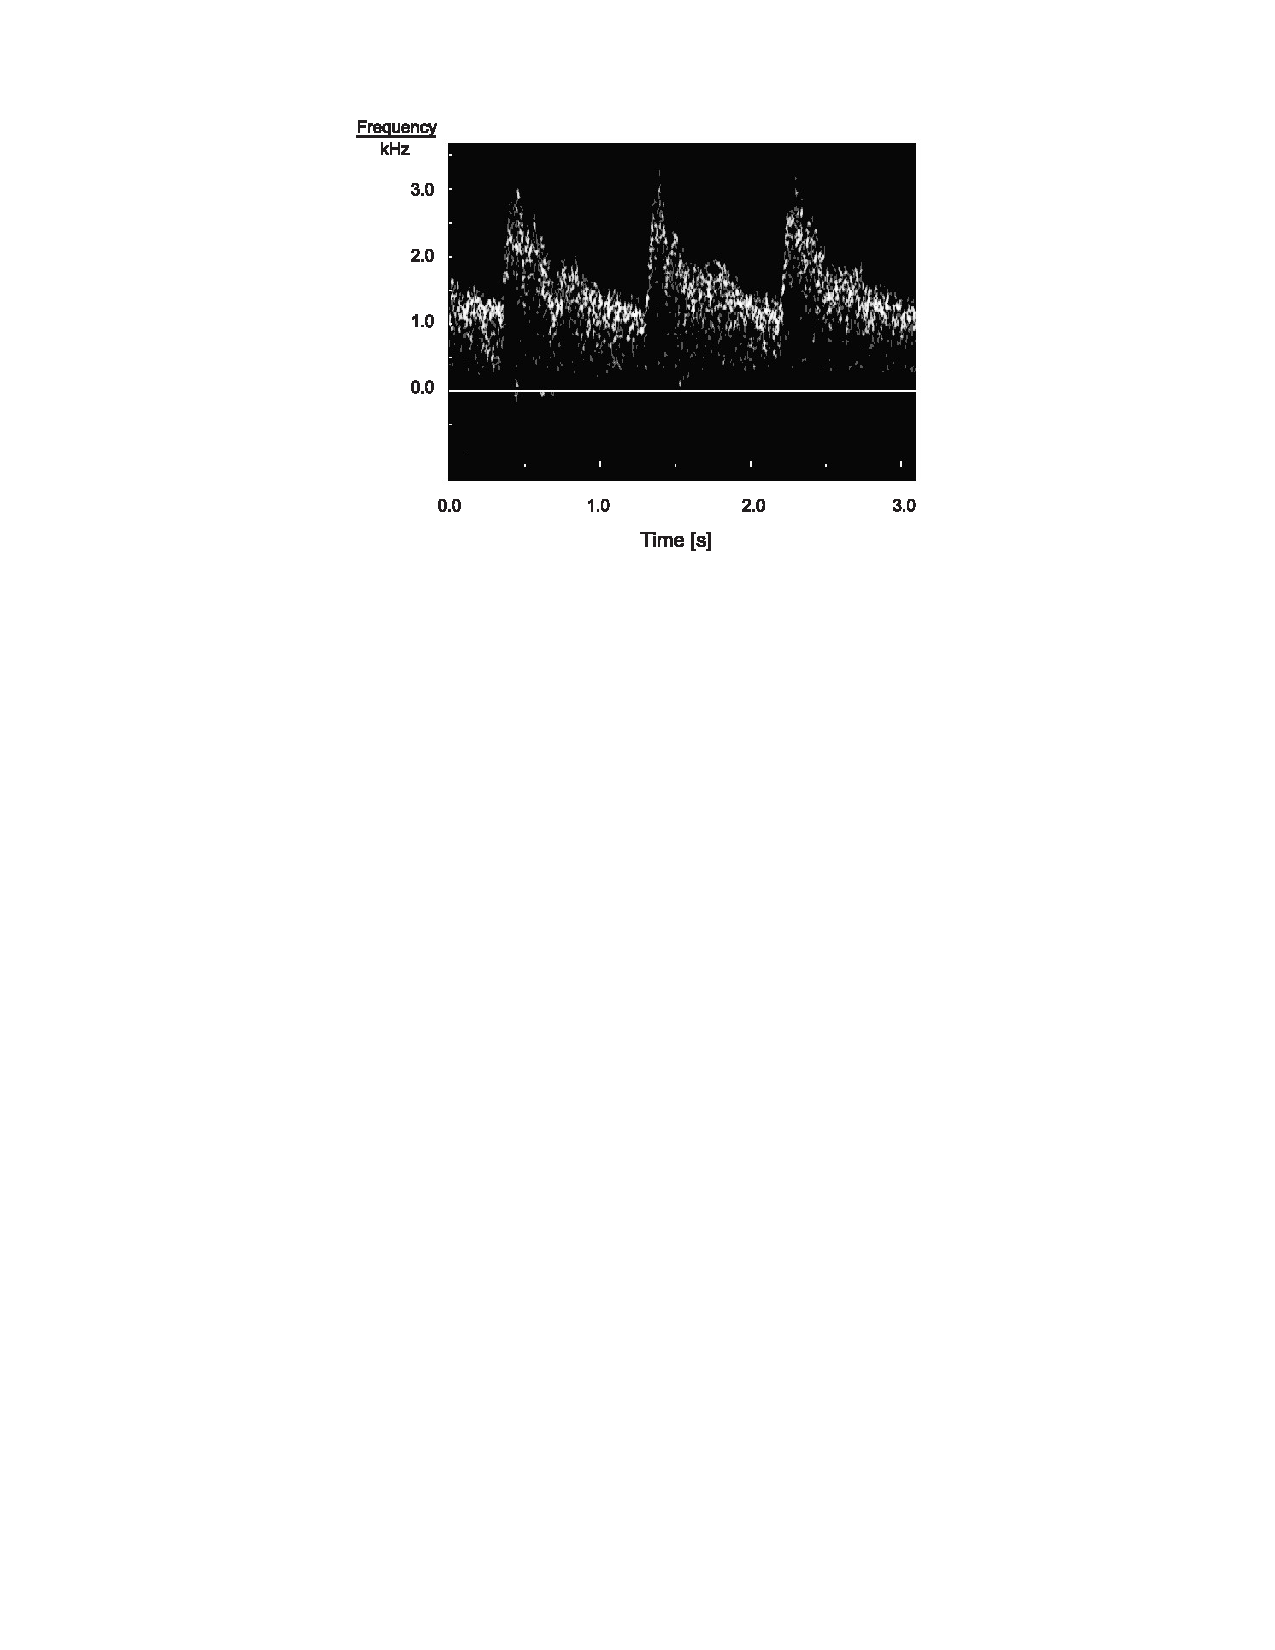
\includegraphics[width=.8\textwidth]{Figures/2_estimation_sonogram_cph.pdf}
	\caption[Arterial sonogram with time-frequency and Doppler shift]{Arterial sonogram with time-frequency and Doppler shift \cite{JensenUltrasoundBook}}
	\label{fig:2_estimation_sonogram_cph}
\end{figure}

Given that the frequency volume of the received signal is similar to the blood's velocity distribution, the Fourier transform of the received signal can be used to obtain velocity. The spectrogram, usually erroneously known as the Doppler spectrum, can be created by saving the \gls{psd} together. The \gls{psd} is calculated for each of the components that make up the received signal in order to accomplish this. A quadrature-demodulated signal is used to display both positive and negative frequencies. When these spectra are shown side by side, the evolution of the velocity distribution can then be seen. Sonography of an artery is displayed in \cref{fig:2_estimation_sonogram_cph}.
